%!TEX root = ../dokumentation.tex

\chapter{Umsetzung}\label{cha:Umsetzung}
<Allgemeine Beschreibung des Inhalts des Kapitels.>

\section{Infrastruktur \& Prozesse}
Vor Beginn der Entwicklung werden im folgenden die Umgebung, in welcher die Applikation später ausgeführt werden soll, sowie der Anwendungsprozess, genauer definiert. 

<Weitere Einführung in das Kapitel bzw. aktuelle überarbeiten>

\subsection{Beschreibung der Infrastruktur}
<...Einleitung/überleitung zur beschreibung der infrastruktur>

Alle Server (sowohl Web- wie auch Appserver), schreiben ihre jeweiligen Logfiles auf ein \ac{NFS}. Der Infrastrukturserver mounted die entsprechenden Verzeichnisse. Der Server verfügt über eine Hadoop Installation, auf welcher die Applikation ausgeführt wird (siehe \autoref{fig:AufbauInfrastruktur}).

\begin{figure}
	\centering
	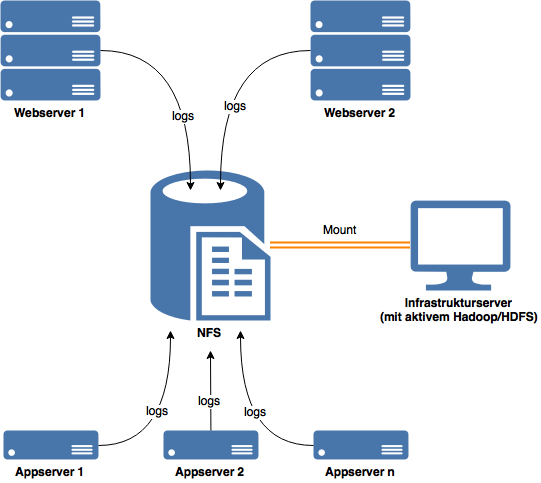
\includegraphics[width=.8\textwidth]{Infrastruktur.png}
	\caption{Aufbau der Infrastruktur}
	\label{fig:AufbauInfrastruktur}
\end{figure}

\subsection{Definition des Anwendungsprozesses}


\begin{figure}
	\centering
	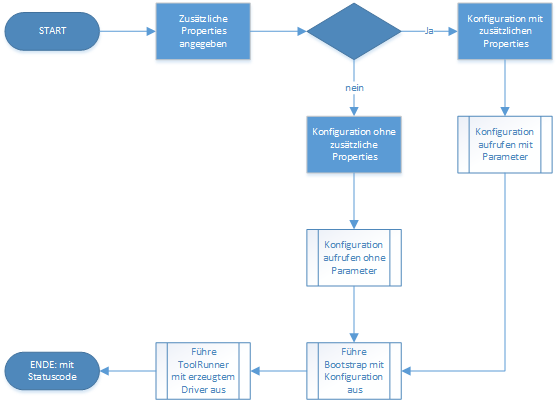
\includegraphics[scale=1]{PAP_Main_main.png}
	\caption{PAP für main Methode der Main Klasse}
	\label{fig:PAP_Main_main}
\end{figure}

<Hier sollte der Prozess der Anwendung geplant werden. wo liegen die Daten? wie findet der zugriff statt? nach welchem schema sind sie abgelegt und benannt? Außerdem sollte klar werden wie die Informationen verarbeitet werden. ein großer map reduce oder eine verkettung mehrerer mapper und reducer? Außerdem muss das ausgabeformat festgelegt werden. Bzw. zwei alternativen. eine für wenn die anwendung performant genug ist um als check skript zu laufen, und eine für den fall das nicht.>

\section{Die Konfigurationsschnittstelle}
Wie bereits bei der Beschreibung des Verarbeitungsprozesses gezeigt wurde, wird direkt nach dem Start der Anwendung eine Initialisierung vorgenommen. Hierbei soll die Umgebung so konfiguriert werden, dass die gewünschte Analyse durch die Anwendung ohne Probleme vorgenommen werden kann.

Die Konfiguration der Anwendung wird durch Dateien vom Typ \textit{.properties} vorgenommen. Diese werden von Java vollständig unterstützt. Für die Interpretation der Konfigurationsdateien wird auf die Klasse \textit{java.util.Properties} zurückgegriffen. Die Funktionsweise der Properties wird im folgenden genauer betrachtet.

\subsection{Aufbau von Properties}
Die Konfigurationswerte werden in Properties Dateien als Schlüssel-Wert-Paare gespeichert. Die Trennung kann hierbei durch einen Doppelpunkt oder Gleichheitszeichen erfolgen. Des weiteren ist es möglich, Platzhalter bei den Werten zu definieren, welche später durch Variablen ersetzt werden können. Außerdem ist es möglich, zum besseren Verständnis, die Datei um Kommentare zu erweitern. Jede Zeile, welche mit einem Hash oder Ausrufezeichen beginnt, wird als Kommentar gesehen, und von der Anwendung nicht interpretiert. \autoref{lis:AuszugDefaultProperties} zeigt einen Auszug aus der \textit{default.properties} Datei. \\

\begin{lstlisting}[language=Bash,caption=Auszug aus default.properties,label=lis:AuszugDefaultProperties]
###
# Default properties for Logfileanalyzer.
# Properties can be extended by user defined properties.
# Never change this file to fit one case.
#

# Set mode for execution (DEBUG, TEST, LIVE)
lfa.runmode         : DEBUG

# Runtime properties
lfa.logger.handlers : {0}

[...]
\end{lstlisting}

Grundsätzlich sind alle Konfigurationen vom Typ \textit{String}. Es ist, nativ, nicht möglich, direkt einen Wert in einem anderen Datentyp zu definieren. Falls eine Typenkonvertieren notwendig ist, muss diese manuell durchgeführt werden.

In Java stellt die Klasse \textit{Properties}, welche teil des \textit{java.util} Paketes ist, alle benötigten Methoden bereit. Um die Konfiguration der Anwendung zu vereinfachen, wurde die Klasse \textit{LFAConfiguration}\footnote{Der Name \textit{LFAConfiguration} wurde bewusst gewählt, da der Name \textit{Configuration} bereits von einer Klasse des Hadoop Frameworks verwendet wird.} im Paket \textit{com.hszuesz.logfileanalyzer} erzeugt. Diese leitet sich aus der Klasse \textit{Properties} ab, und stellt Erweiterungen zum einlesen mehrerer Konfigurationsdateien bereit. Dies ist notwendig, um eine stufenweise Konfiguration der Anwendung zu realisieren.

Da die Anwendung später innerhalb des Hadoop Frameworks ausgeführt wird, müssen die Konfigurationsdateien ein Teil der, durch Maven erzeugten, JAR-Datei sein. Dies wird durch eine Ergänzung in der \textit{pom.xml} innerhalb des \textit{build} Knotens sichergestellt (siehe \autoref{lis:POMErgänzung}). \\

\begin{lstlisting}[language=XML,caption=pom.xml Ergänzung für Konfigurationsdateien,label=lis:POMErgänzung]
[...]
<resources>
	<resource>
		<directory>conf</directory>
		<includes>
			<include>*.properties</include>
		</includes>
	</resource>
</resources>
[...]
\end{lstlisting}

\subsection{Beschreibung der Konfigurationsstufen}
Die Konfiguration der Anwendung wird in drei Stufen durchgeführt. Dies soll die Komplexität der Konfigurationsdateien reduzieren, indem die individuellen Anpassungen für jede Ausführung des Programms gekapselt, und immer gleiche Einstellungen ausgelagert werden.

Die erste Stufe bilden die sog. Core-Properties, welche in der Datei \textit{core.properties} hinterlegt sind. Wie der Name bereits erkennen lässt, handelt es sich hierbei um Grundlegende Einstellungen, welche den Kern der Anwendung beeinflussen. Dazu gehört z.B. die Konfiguration der verschiedenen \textit{RUNMODES} oder Pfade zu weiteren wichtigen Dateien, wie den Default- oder Logger-Properties. Ein überschreiben dieser Einstellungen ist nicht möglich.

Die zweite Stufe bildet die Defaults. Hier werden alle Konfigurationen vorgenommen, welche für eine Standardausführung der Anwendung benötigt werden. Alle Einstellungen, welche in der \textit{defaults.properties} Datei hinterlegt sind, können durch den Anwender verändert werden.

Die dritte und letzte Stufe bilden die User-Properties. Beim Start der Anwendung kann der Pfad zu einer individuellen Properties-Datei übergeben werden. In dieser können die Einstellungen, welche durch die Defaults vorgenommen wurden, ergänzt und  überschreiben werden.

Der Prozess für die Verarbeitung der einzelnen Stufen wird im \ac{PAP} der \textit{LFAConfiguration} verdeutlicht, welcher im Anhang zu finden ist.\footnote{\ac{PAP} für \textit{LFAConfiguration} im Anhang, S. \pageref{subsec:PAPLFAConfiguration}}

%<Beschreibung wie Properties programmiert werden. Wie werden diese in der Anwendung umgesetzt? Welche Rolle spielen Properties für den generischen Teil der Anwendung?>

\subsection{Logger Konfiguration}
<Beschreibung wie der Logger in Java funktioniert und wie dieser hier eingesetzt wird. Speziell die Konfiguration über die logger.properties datei hervorheben.>

%\section{Grundlagen für Datenverarbeitung}
%<Beschreibung der Entwicklung für die Grundlagen zur Datenverarbeitung. Welche Klassen werden dabei verwendet? Welches System liegt dahinter? Warum dieses System? Dabei nicht nur auf die Speicherung von Daten eingehen sondern auch auf das Lesen von Dateien.>

%\section{Bestimmung des Aufbaus der Logfiles}
%<Wie sehen die Logfiles aus? Welche Formate haben sie? Welche rolle spielen diese bei der Datenverarbeitung? Welche Informationen sind die richtigen Informationen?>

\section{Implementierung von MapReduce}
Nachdem alle Grundlagen der Anwendung fertiggestellt wurden kann mit der Entwicklung des Kernstückes begonnen werden, der Implementierung von MapReduce. Zunächst wird der Verarbeitungsprozess innerhalb des MapReduce Modells beschrieben. Im Anschluss werden einzelne Module genauer betrachtet.

Um dem generischen Anforderungen der Anwendung gerecht zu werden, ist ein Verständnis des modularen Aufbaus des Modells, für die Entwicklung der individuellen Anpassungen, von entscheidender Bedeutung. 

\subsection{Datenfluss in MapReduce}
Ein MapReduce Job beginnt mit der Übertragung der Daten an die Klasse \textit{InputFormat}. Diese teilt die Daten nach einer vorgegebenen Größe\footnote{Standardgröße für \textit{FileInputFormat} beträgt 64 \ac{MB}. Dieser Wert kann durch setzen der Einstellung \textit{mapred.min.split.size} verändert werden. Die Angabe erfolgt in Bytes.}. Jeder erzeugte \textit{Split} wird von einem \textit{Mapper} verarbeitet. Dabei werden die Daten mit dem \textit{RecordReader} aufbereitet, welcher die initialen Schlüssel-Wert-Paare ermittelt. Im Anschluss werden diese an die \textit{Map}-Funktion weitergegeben. Die einzelnen \textit{Splits} werden parallel verarbeitet.

Erst wenn alle \textit{Mapper} die Verarbeitung abgeschlossen haben, folgt die Partitionierung und Sortierung der neuen Schlüssel-Wert-Paare. Die Sortierten Paare werden den \textit{Reducern} übergeben.

Abschließend wird das Ergebnis der Analyse an eine Instanz der Klasse \textit{OutputFormat} übergeben, welche das Resultat aufbereitet und im \ac{HDFS} ablegt. \autoref{fig:DatenflussMapReduce} stellt den Datenfluss zur Verdeutlichung grafisch dar.

\begin{figure}[h]
	\centering
	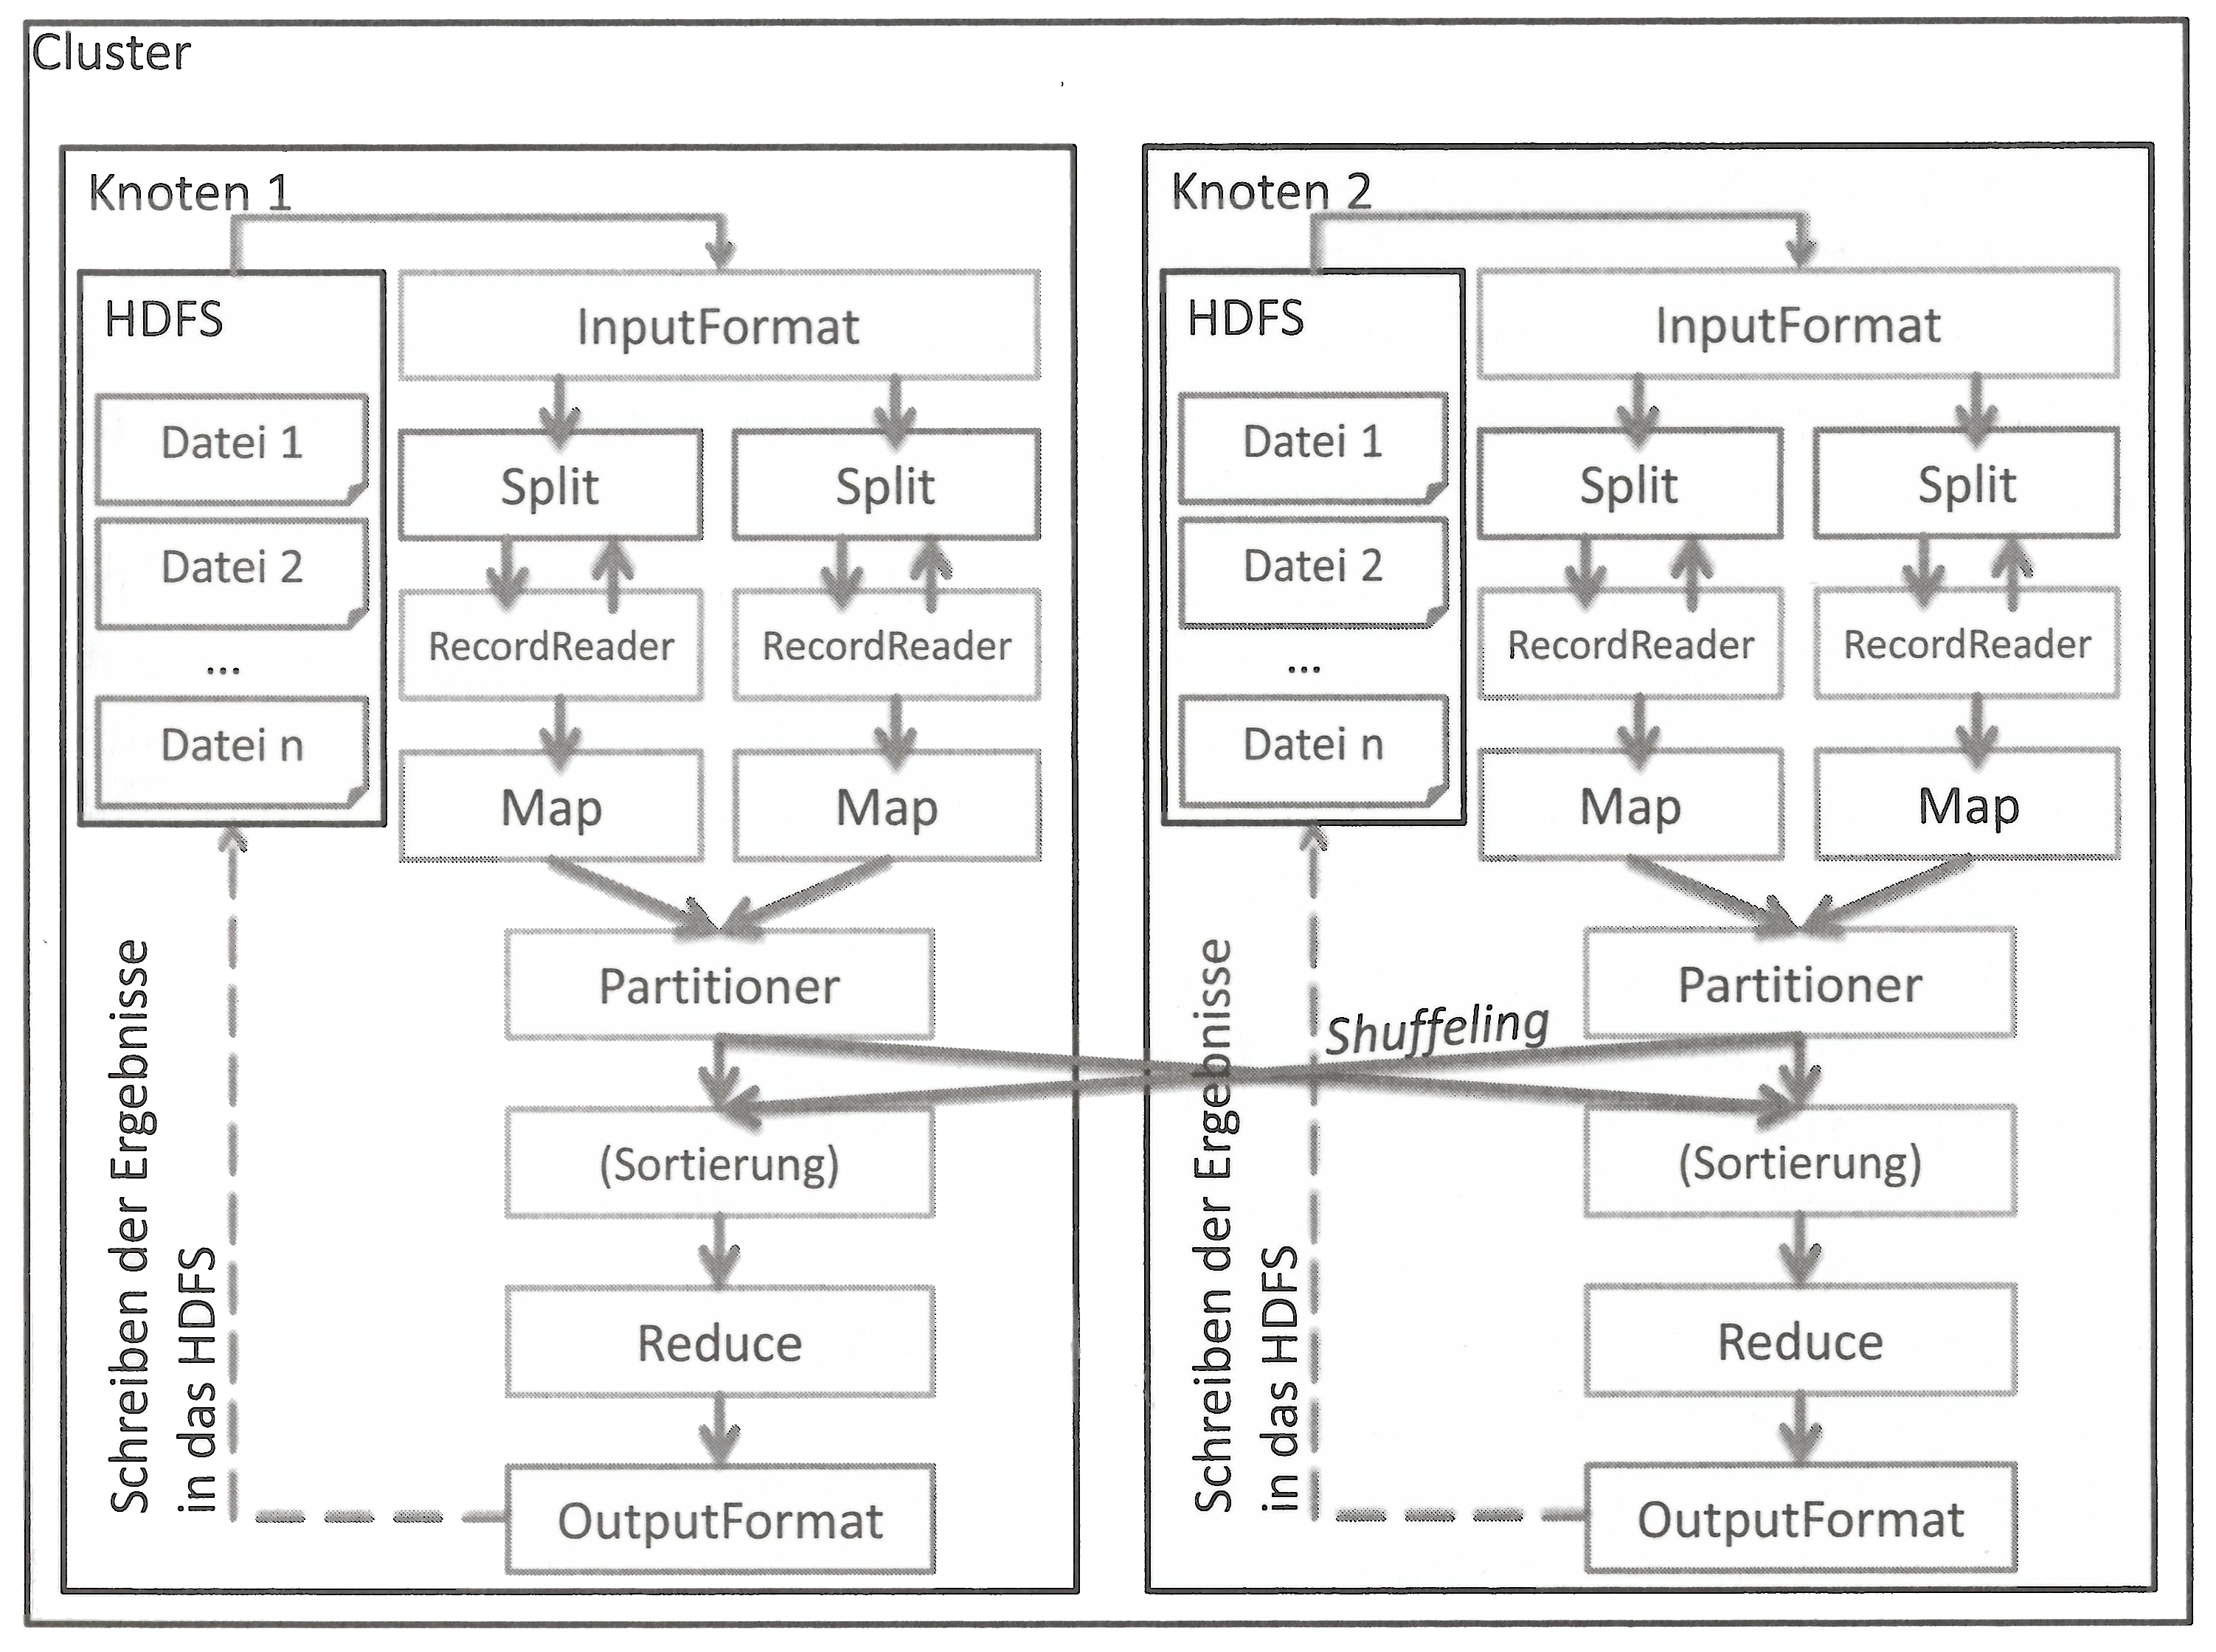
\includegraphics[width=1\textwidth]{MapReduceDatenfluss.png}
	\caption{Datenfluss in MapReduce\footnotemark}
	\label{fig:DatenflussMapReduce}
\end{figure}
\footnotetext{\cite[S. 111]{Freiknecht.2014}}

Die einzelnen Module, sowie deren Implementierung in der Anwendung, werden in den nächsten Abschnitten beschrieben, mit Ausnahme der Module \textit{Partitioner} und der \textit{Sortierung}, da diese keine Anpassungen benötigen.

Zusätzlich zu den Modulen von MapReduce, werden vorab die Klassen \textit{Bootstrap} und \textit{Driver} beschrieben. Diese gehören nicht direkt in das Modell von MapReduce sondern sind Teil der Initialisierung der Anwendung selbst.

\subsection{Funktion von Bootstrap \& Driver}
Durch den generischen Ansatz der Anwendung muss jeder Programmlauf initialisiert werden (auch als \gls{Bootstrapping} bezeichnet). Dies wird durch die Methode \textit{init} der Klasse \textit{Bootstrap} durchgeführt. Die zuvor erstellte Instanz der Klasse \textit{LFAConfiguration} wird hierfür an die Methode übergeben. Basierend auf den gesetzten Properties wird eine Instanz der Klasse \textit{Driver} erzeugt (siehe \autoref{lst:BootstrapInit} oder \ac{PAP}\footnote{\ac{PAP} für \textit{Bootstrap:init() im Anhang, S. \pageref{subsec:PAPBootstrapInit}}}).

Dem \textit{Driver} werden zunächst alle Klassen mitgeteilt, welche zur Ausführung eines Jobs essentiell notwendig sind. Hierzu gehören die Klassen für \textit{InputFormat}, \textit{OutputFormat}, \textit{OutputKey}, \textit{OutputValue}, \textit{Mapper} und \textit{Reducer}. Die gesetzten Werte sind vom Typ \textit{Class<?>}. Es werden keine Instanzen der Klassen erzeugt. Ebenfalls notwendig für die Ausführung eines Jobs ist das Setzen eines Namens.

Zuletzt wird eine Iteration über alle Schlüssel der Konfiguration durchgeführt, um zusätzliche Properties an den \textit{Driver} zu übergeben. Diese erweiterten Einstellungen werden vor Ausführung des Jobs in eine Instanz der Klasse \textit{org.apache.hadoop.conf.Configuration} geschrieben. Bei diesen Properties handelt es sich um Einstellungen, welche von den einzelnen Modulen des MapReduce Modells verwendet werden (z.B. ein regulärer Ausdruck für die \textit{Mapper} Klasse).\\

\begin{lstlisting}[language=Java,caption=Auszug der Methode \textit{Bootstrap:init()},label=lst:BootstrapInit]
public static Driver init(LFAConfiguration objConfiguration) {
	[...]
	// Set class to use for InputFormat
	objDriver.setClsInputFormatClass(Class.forName(objConfiguration.getProperty("lfa.driver.input.format")));
	
	// Set classes regarding the output
	objDriver.setClsOutputFormatClass(Class.forName(objConfiguration.getProperty("lfa.driver.output.format")));
	objDriver.setClsOutputKeyClass(Class.forName(objConfiguration.getProperty("lfa.driver.output.key")));
	objDriver.setClsOutputValueClass(Class.forName(objConfiguration.getProperty("lfa.driver.output.value")));
	
	// Set classes for mapper and reducer
	objDriver.setClsMapperClass(Class.forName(objConfiguration.getProperty("lfa.driver.mapper")));
	objDriver.setClsReducerClass(Class.forName(objConfiguration.getProperty("lfa.driver.reducer")));
	
	// Set job name
	objDriver.setStrJobName(objConfiguration.getProperty("lfa.driver.job.name"));
	
	Set<String> setKeys = objConfiguration.stringPropertyNames();
	
	// Extract additional properties for the MapReduce job
	for (String strKey : setKeys) {
		if (strKey.contains("lfa.mapper.") || strKey.contains("lfa.reducer.") || strKey.contains("lfa.driver.add.")) {
			objDriver.setAdditionalConfiguration(strKey, objConfiguration.getProperty(strKey));
		}
	}
	[...]
}
\end{lstlisting}

Die Klasse \textit{Driver} leitet sich von \textit{org.apache.hadoop.conf.Configured} ab und implementiert das Interface \textit{org.apache.hadoop.util.Tool}. Von der Klasse \textit{Configured} werden alle notwendigen Methoden und Attribute geerbt, welche für die Verwendung der, durch das Hadoop Framework gestellte und interpretierte, Konfiguration notwendig sind. Durch das Interface wird wiederum die Implementierung der Methode \textit{run()} vorgegeben.

Diese Methode, welche später durch den \textit{ToolRunner} aufgerufen wird, Erstellt und Konfiguriert einen neuen Job, um diesen auszuführen und seinen Statuscode zurück zu geben. Hier werden alle, durch die \textit{Bootstrap:init()} Methode gesetzten Einstellungen, an den Job übergeben. Dieser Umweg ist notwendig, da ein Job mit einer Instanz von \textit{import org.apache.hadoop.conf.Configuration} erzeugt werden muss. Diese steht erst nach Ausführung durch den \textit{ToolRunner} zu Verfügung.

Dieser Konfigurationsklasse werden ebenfalls die zusätzlichen Einstellungen übergeben, sofern diese vorhanden sind. Das übergebene Array enthält die Pfade für den Input und Output des Jobs, welche der Klasse \textit{FileInputFormat} und \textit{FileOutputFormat} hinzugefügt werden. \autoref{lst:AuszugRunMethode} zeigt einen Auszug der \textit{run} Methode (siehe auch \ac{PAP}\footnote{\ac{PAP} für \textit{Driver.run()} im Anhang, S. \pageref{subsec:PAPDriverRun}}) \\

\begin{lstlisting}[language=Java,caption=Auszug der \textit{run()} Methode,label=lst:AuszugRunMethode]
public int run(String[] arrArguments) throws Exception {
	Configuration objConf = this.getConf();
	
	if (this.mapAdditionalConfigurations.size() > 0) {
		for (String strKey : this.mapAdditionalConfigurations.keySet()) {
			objConf.set(strKey, this.mapAdditionalConfigurations.get(strKey));
		}
	}
	
	Job objJob = new Job(objConf, this.strJobName);
	
	[...]
	
	FileInputFormat.addInputPath(objJob, new Path(arrArguments[0]));
	objJob.setInputFormatClass(this.clsInputFormatClass);
	
	FileOutputFormat.setOutputPath(objJob, new Path(arrArguments[1]));
	objJob.setOutputFormatClass(this.clsOutputFormatClass);
	
	return objJob.waitForCompletion(true) ? 0 : 1;
}
\end{lstlisting}

\subsection{Einblick in die InputFormat Klasse}


\subsection{Der RecordReader}


\subsection{Mapper und Reducer}
Die durch den \textit{RecordReader} erzeugten Schlüssel-Wert-Paare werden an den Mapper weiter gegeben. Die Aufgabe des \textit{Mappers}, ist die weiterverarbeitung und genauere Interpretation/Analyse der Paare.

Wichtig ist hierbei die unterscheidung zwischen der Aufgabe des \textit{RecordReader} und \textit{Mapper}. Beider wandeln gegebene Informationen in Schlüssel-Wert-Paare um. Die durch den \textit{RecordReader} erzeugten Paare sind als die Datensätze zu sehen, welche durch den Mapper analysiert werden sollen.

Diese Trennung muss bei der Entwicklung unter allen Umständen beachtet werden. Der \textit{RecordReader} darf nicht die Aufgaben des \textit{Mapper} übernehmen.

Die Interpretation der Daten kann auf unterschiedlichste weise erfolgen. Die Auswertung ist dabei immer an den zu verarbeitenden Datentyp angepasst. Analysiert werden können alle formen von Daten (Numerisch, Alphanumerisch oder binäre Daten).

\subsubsection{Implementierung individueller Mapper}
Alle Mapper müssen sich von der Klasse \textit{org.apache.hadoop.mapreduce.Mapper} ableiten. Bei der Klassendefinition muss ebenfalls die Angabe der \glspl{Generic} erfolgen. Der Mapper wird in der Hadoop 2.7.1 \ac{API} der Apache Software Foundation Definiert mit \textit{Class Mapper<KEYIN,VALUEIN,KEYOUT,VALUEOUT>}. Die \glspl{Generic} geben für die Schlüssel-Wert-Paare, sowohl vom Input (\textit{KEYIN}, \textit{VALUEIN}) wie auch für den Output (\textit{KEYOUT}, \textit{VALUEOUT}), die Datentypen an.\footcite[Vgl.][]{ApacheHadoopApiDokuMapper.2015}

\autoref{lst:DefinitionPatternMapper} zeigt die Definition der für diese Anwedung programmierten Klasse \textit{PatternMapper}, mit den entsprechenden Generics innerhalb der spitzen Klammern. Diese erwartet als Input ein Schlüssel-Wert-Paar, bei welchem der Schlüssel ein beliebiges Objekt und der Wert ein Objekt des Typs \textit{org.apache.hadoop.io.Text} repräsentiert. Das Inputpaar wird durch die Methode \textit{map()} in ein Schlüssel-Wert-Paar mit Schlüsseltyp \textit{org.apache.hadoop.io.Text} und Werttyp \textit{org.apache.hadoop.io.IntWritable} umgewandelt. \\

\begin{lstlisting}[language=Java,caption=Deklaration \textit{PatternMapper} mit Generics,label=lst:DefinitionPatternMapper]
public class PatternMapper extends Mapper<Object,Text,Text,IntWritable>
\end{lstlisting}

Der \textit{PatternMapper} Analysiert den übergebenen Wert anhand eines in der Konfiguration definierten regulären Ausdrucks. Dieser kann alle Daten analysieren, welche durch \acp{DEA} oder \acp{NEA} erkannt werden können, d.h., dass die Daten mit einer \textit{Grammatik} vom \textit{Typ 3} der Chomsky-Hierarchie interpretiert werden können. Diese wird von Ulrich Hedtstück wie folgt definiert:

Sei $G = (V_N, V_T, P, S)$ eine \textit{Grammatik}, mit der endlichen, nichtleeren Mengen $V = V_N \cup V_T$, wobei $V_N$ die Menge aller \textit{Variablen} (\textit{nichtterminalen Symbole}) und $V_T$ die Menge aller \textit{terminalen Symbole} (\textit{Terminale}) ist, einer endlichen Menge $P$ von \textit{Regeln} (\textit{Produktionen}) der Form $\alpha$ \textrightarrow $\beta$ (mit $\alpha \in (V_N \cup V_T)^+$ und $\beta \in (V_N \cup V_T)^*$) und dem \textit{Startsymbol} $S \in V_N$. 

$G$ ist vom \textit{Typ 3} oder \textit{regulär}, wenn es eine Produktion der Form \textit{A} \textrightarrow \textit{aB}, oder \textit{A} \textrightarrow \textit{a} hat, wobei $A, B \in V_N$, $a \in V_T$, mit der Ausnahme \textit{S} \textrightarrow $\varepsilon$, wobei \textit{S} nie auf der rechten Seite einer Produktion stehen darf.\footcite[Vgl.][S. 25 u. 32]{Hedtstueck.2012}

Eine \textit{Grammatik} von diesem Typ kann immer in einen regulären Ausdruck umgewandelt werden. Der \textit{PatternMapper} ermittelt anhand dieses Ausdrucks den Schlüssel innerhalb des ihm übergebenen Wertes. Der reguläre Ausdruck muss über mindestens eine definierte Gruppe verfügen, da diese letztendlich als Schlüssel verwendet wird. Wenn dieser gefunden wird, kann als Ergebnis ein Schlüssel-Wert-Paar dem aktuellen \textit{Mapper-Context}, mittels der Methode \textit{write()}, mit einem Wert von $1$, hinzugefügt werden. Wird keine Übereinstimmung gefunden, kann der Eintrag, durch das Setzen einer entsprechenden Konfiguration auf den Wert \textit{SKIP}, ignoriert werden. Anderenfalls wird \textit{NA} als Schlüssel verwendet. \autoref{lst:MethodeMap} zeigt die Methode \textit{map()} des \textit{PatternMappers}. \\

\begin{lstlisting}[language=Java,caption=Methode \textit{map()} der Klasse \textit{PatternMapper},label=lst:MethodeMap]
public void map(Object objKey, Text objValue, Mapper.Context objContext) throws IOException, InterruptedException {
	Configuration	objConf						= objContext.getConfiguration();
	Pattern				objKeyPattern			= Pattern.compile(objConf.get([...]));
	String				strNoMatchAction	= objConf.get([...]);

	String 	strLine 		= objValue.toString();
	Matcher	objMatcher	= objKeyPattern.matcher(strLine);

	if (objMatcher.find()) {
		this.objTmpKey.set(objMatcher.group(1));
		objContext.write(this.objTmpKey, PatternMapper.objOne);
	} else {
		if ("SKIP".equals(strNoMatchAction)) {
			Logger.getLogger(PatternMapper.class.getName()).log(Level.WARNING, [...]);
		} else {
			Logger.getLogger(PatternMapper.class.getName()).log(Level.WARNING, [...]);
			this.objTmpKey.set("NA");
			objContext.write(this.objTmpKey, PatternMapper.objOne);
		}
	}
}
\end{lstlisting}

Wie in \autoref{fig:DatenflussMapReduce} gezeigt wird, werden die durch den \textit{Mapper} erzeugten Schlüssel-Wert-Paare, nach deren Partitionierung/Sortierung, an den \textit{Reducer} weitergegeben.

\subsubsection{Implementierung individueller Reducer}
Die Definition der \textit{Reducer} Klasse, in der Hadoop 2.7.1 \ac{API} ähnelt stark der des \textit{Mappers} mit \textit{Class Reducer<KEYIN,VALUEIN,KEYOUT,VALUEOUT>}.\footcite[Vgl.][]{ApacheHadoopApiDokuReducer.2015} Die Generics haben die gleiche Bedeutung wie die des \textit{Mappers}.

\autoref{lst:DefinitionCountReducer} zeigt die Definition des für die Anwendung programmierten \textit{CountReducer}.  \\

\begin{lstlisting}[language=Java,caption=Deklaration \textit{CountReducer} mit Generics,label=lst:DefinitionCountReducer]
public class CountReducer extends Reducer<Text, IntWritable, Text, IntWritable>
\end{lstlisting}

Der \textit{CountReducer} summiert alle im \textit{Mapper} gesetzten Werte für einen gegebenen Schlüssel auf und schreibt das Ergebnis wieder in den entsprechenden Context. \autoref{lst:MethodeReduce} zeigt die \textit{reduce()} Methode der Klasse \textit{CountReducer}. Im gegensatz zur \textit{map()} Methode, bekommt der \textit{Reducer} ein Array von werten übergeben. \\

\begin{lstlisting}[language=Java,caption=Methode \textit{reduce()} der Klasse \textit{CountReducer},label=lst:MethodeReduce]
public void reduce(Text objKey, Iterable<IntWritable> arrValues, Context objContext) throws IOException, InterruptedException {
	int lngSum = 0;

	for(IntWritable objValue : arrValues) {
		lngSum += objValue.get();
	}

	this.objTotal.set(lngSum);

	objContext.write(objKey, this.objTotal);
}
\end{lstlisting}

Der \textit{Reducer} kann auch andere Aufgaben übernehmen. Die naheliegensten Funktionen sind arithmetische Operationen wie die Berechnung eines arithmetischen Mittels, des Medians oder minimal/maximal Werte für einen Schlüssel.

Je nach Analyse müssen unterschiedliche \textit{Mapper} und/oder \textit{Reducer} programmiert werden. Die zu verwendenden Klassen sind über die entsprechenden Properties konfigurierbar.

\subsection{Betrachtung von alternativen Mappingverfahren}


\section{Ausführungsdatei Logfileanalyzer.sh}\label{sec:Ausführungsdatei}


\begin{lstlisting}[language=Bash,caption=Ausführungsdatei Logfileanalyzer.sh,label=lis:Logfileanalyzer.sh]
#!/bin/bash
#Load config
. $1/config.cfg
#Cleanup input direktory on dfs
/bin/hdfs dfs -rm -r -skipTrash input/*
#Delete output directory on dfs
/bin/hdfs dfs -rm -r -skipTrash output
#Put input files on dfs
/bin/hdfs dfs -put $MAP_REDUCE_INPUT input
mkdir $MAP_REDUCE_OUTPUT
if [ $MAP_REDUCE_USE_USER_PROPERTIES == true ]
then
	#Export HADOOP_OPTS to pass user properties file
	export HADOOP_OPTS="-Dlfa.userconf=$1/$MAP_REDUCE_USER_PROPERTIES"
fi
if [ $MAP_REDUCE_USE_LOG == true ]
then
	#Use log logfile
	echo "Log file wird verwendet"
	/bin/hadoop jar $1/$MAP_REDUCE_JAR $MAP_REDUCE_MAIN input output 2> $MAP_REDUCE_LOGFILE
else
	echo "Kein Logfile"
	/bin/hadoop jar $1/$MAP_REDUCE_JAR $MAP_REDUCE_MAIN input output
fi
if [ $MAP_REDUCE_USE_USER_PROPERTIES == true ]
then
	#Unset HADOOP_OPTS after apllication finished
	export HADOOP_OPTS=""
fi
#Get output from dfs
/bin/hdfs dfs -get output/* $MAP_REDUCE_OUTPUT
if [ $MAP_REDUCE_DISPLAY_OUTPUT == true ]
then
	cat ${MAP_REDUCE_OUTPUT}/*
fi
\end{lstlisting}

<Beschreiben der Bash Datei, durch welche der job (Jar) ausgeführt wird. Beschreiben der einzlenen Schritte und der configuration>

\section{Anwendungstest \& Auswertung der Ergebnisse}
Bevor die Anwendung in den produktiven Betrieb über gehen kann, wird sie unter exakt spezifizierten Bedingungen getestet. Die so durchgeführten Tests sollen Aufschluss über die Leisung der Anwendung geben.

\subsection{Durchführung der Tests}
Für die Tests werden eine Reihe von Logfiles in unterschiedlichen größen bereitgestellt. Diese enthalten $10$ bis $10^7$ Einträgen. Jedes Logfile wird 10 mal durch die Anwendung analysiert und die Laufzeit protokolliert. \autoref{lis:PropertiesAnwendungstest} zeigt die für die Tests verwendete Konfiguration. \\

\begin{lstlisting}[language=Java,caption=Properties für Anwendungstest,label=lis:PropertiesAnwendungstest]
lfa.runmode              : DEBUG

lfa.driver.mapper        : com.hszuesz.logfileanalyzer.mapper.PatternMapper
lfa.driver.reducer       : com.hszuesz.logfileanalyzer.reducer.CountReducer

lfa.driver.input.format  : org.apache.hadoop.mapreduce.lib.input.TextInputFormat

lfa.driver.output.key    : org.apache.hadoop.io.Text
lfa.driver.output.value  : org.apache.hadoop.io.IntWritable
lfa.driver.output.format : org.apache.hadoop.mapreduce.lib.output.TextOutputFormat

lfa.driver.job.name      : Laufzeittest webadapter.log

lfa.mapper.pattern.key   : \\] ([A-Z]{4,5})
lfa.mapper.nomatchaction : SKIP
\end{lstlisting}

Bei jeder Ausführung des Programms wird das in \autoref{sec:Ausführungsdatei} beschriebene Bash-Script ausgeführt, wodurch die Logfiles vor jede Analyse neu in das \ac{HDFS} übertragen wird. Dies ist notwendig, da bei jedem Upload die Datenblöcke neu geschrieben werden müssen, um ein verfältschtes ergebniss durch Caching zu vermeiden.

\autoref{fig:Streudiagram} zeigt die einzelnen Testläufe als Datenpunkte, \autoref{tbl:DurchschnittlicheLaufzeiten} die arithmetischen Mittelwerte für die einzelnen Logfilegrößen.

\begin{figure}
	\centering
	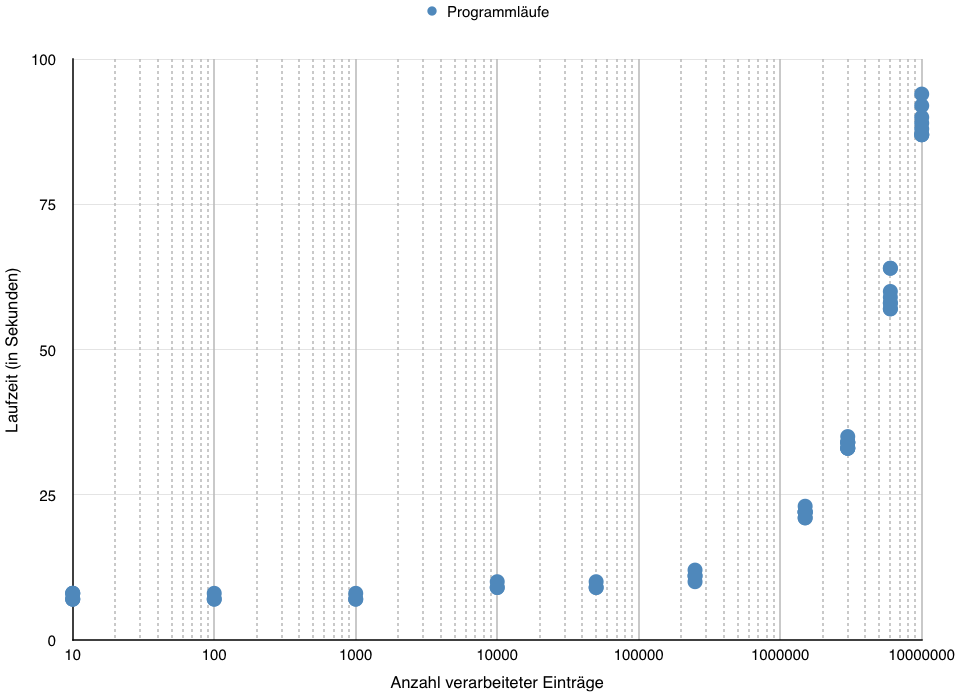
\includegraphics[width=1\textwidth]{ErgebnisAnwendungstest.png}
	\caption{Streudiagram der Laufzeiten}
	\label{fig:Streudiagram}
\end{figure}

\begin{table}
	\centering
	\begin{tabular}{| r | l | r | r |}
		\hline
		\rowcolor[HTML]{3531FF} 
		\multicolumn{1}{|l|}{\cellcolor[HTML]{4F88BB}{\color[HTML]{FFFFFF} {\bf \#}}} & \multicolumn{1}{l|}{\cellcolor[HTML]{4F88BB}{\color[HTML]{FFFFFF} {\bf Anzahl Einträge}}} & \multicolumn{1}{l|}{\cellcolor[HTML]{4F88BB}{\color[HTML]{FFFFFF} {\bf Dateigröße}}} & \multicolumn{1}{l|}{\cellcolor[HTML]{4F88BB}{\color[HTML]{FFFFFF} {\bf Laufzeit}}} \\ \hline
		1 & $10$ & 1,6 \ac{KB} & 7,4 \\  \hline
		2 & $100$ & 17,0 \ac{KB} & 7,1 \\ \hline
		3 & $1000$ & 157,0 \ac{KB} & 7,3 \\  \hline \hline
		4 & $10^4$ & 1,6 \ac{MB} & 9,1 \\  \hline
		5 & $5\times10^4$ & 7,7 \ac{MB} & 9,1 \\  \hline
		6 & $2,5\times10^5$ & 39,0 \ac{MB} & 11,0 \\  \hline
		7 & $1,5\times10^6$ & 231,0 \ac{MB} & 21,7 \\  \hline
		8 & $3\times10^6$ & 461,0 \ac{MB} & 33,7 \\  \hline
		9 & $6\times10^6$ & 921,0 \ac{MB} & 59,5 \\  \hline \hline
		10 & $10^7$ & 1,5 \ac{GB} & 88,9 \\  \hline
	\end{tabular}
	\caption{Durchschnittliche Laufzeiten (in Sekunden) für gegebene Datenmenge}
	\label{tbl:DurchschnittlicheLaufzeiten}
\end{table}

Die visuelle Darstellung lässt einen stärkeren Zusammenhang zwischen den beiden größen $x$ und $y$ vermuten. Aus diesem grund werden, die durch den Anwendungstest erhobenen Daten, genauer betrachtet.

Da die Tests auf der in \autoref{sec:InstallationHadoop} erwähnten \ac{VM} durchgeführt wurden, können die im folgenden getroffenen Aussagen vom späteren produktiven Betrieb abweichen. Aus diesem Grund sollten vor Inbetriebnahme der Anwendung weitere Tests auf einem System ähnlich dem Produktivsystem durchgeführt werden, um aussagekräftigere Daten zu erhalten.

\subsection{Analyse der Laufzeiten}
Die im Anwendungstest erhobenen Laufzeiten sollen nun weiter Analysiert werden. Hierfür soll zunächst das Ausmaß des \textit{linearen} Zusammenhangs zwischen der Anzahl der verarbeiteten Einträge und der Laufzeit ermittelt werden. Gerald und Susanne Teschl definieren die, nach dem englischen Mathematiker Karl Pearson (1857 - 1936) benannte, Kennzahl wie folgt:

\flqq Gegeben seien die Wertepaare $(x_1,y_1), \dots,(x_n,y_n)$, wobei nicht alle $x_i$ gleich sind bzw. nicht alle $y_i$ gleich sind. Die Zahl
\begin{equation*}
r_{xy} = \frac{s_{xy}}{s_x \cdot s_y}
\end{equation*} 
heißt \textbf{(empirischer) Korrelationskoeffizient} oder \textbf{Pearson'scher Korrelationskoeffizient}. Dabei ist
\begin{equation*}
s_{xy} = \frac{1}{n-1} \displaystyle\sum_{i=1}^{n} (x_i - \bar{x})(y_i - \bar{y})
\end{equation*}
die \textbf{(empirische) Kovarianz}, $\bar{x}$, $\bar{y}$ sind die arithmetischen Mittelwerte und
\begin{equation*}
s_x = \sqrt{\frac{1}{n-1} \displaystyle\sum_{i=1}^{n} (x_i - \bar{x})^2}, \quad s_y = \sqrt{\frac{1}{n-1} \displaystyle\sum_{i=1}^{n} (y_i - \bar{y})^2}
\end{equation*}
sind die (empirischen) Standardabweichungen der $x_i$ bzw. der $y_i$-Werte.\frqq\footcite[S. 213]{Teschl.2014}

Der Pearson'sche Korrelationskoeffizient liegt immer zwischen $-1$ und $+1$. Je näher $r_{xy}$ an $-1$ oder $1$ liegt, desto genauer konzentrieren sich die Datenpunkte auf einer Geraden. Zudem spricht man bei einem Korrelationskoeffizienten $r_{xy}>0$ von einer \textbf{positiven (linearen) Korrelation}.\footcite[Vgl.][S. 214]{Teschl.2014}

Nach Anwendung der eben definierten Gleichungen auf die, durch den Anwendungstest, ermittelten Werte, ergibt sich ein Wert von $r_{xy} \approx 0,9982$. Daraus folgt eine starke, lineare Korrelation zwischen der Laufzeit und der Anzahl der verarbeiteten Einträge.

Basierend auf dieser Abhängigkeit lässt sich, durch die sog. \textbf{Regressionsanalyse}, eine Funktion bestimmen, mit welcher, die zu erwartende Laufzeit der Anwendung, in Abhängigkeit zur Menge der zu verarbeitenden Daten, approximiert werden kann.

Bei der \textbf{linearen Regression} wird eine Funktion der Form $y = f(x) = kx + d$ gesucht (der sog. \textbf{Regressionsgeraden}), welche der folgenden Definition gerecht wird:

\flqq Die Gerade $f(x) = kx + d$, für die
\begin{equation*}
\displaystyle\sum_{i=1}^{n} (y_i - f(x_i))^2
\end{equation*}
minimal wird, ist gegeben durch
\begin{equation*}
k = r_{xy} \frac{s_y}{s_x}, \quad \quad d = \bar{y} - k\bar{x}.
\end{equation*}
Hier ist $r_{xy}$ der empirische Korrelationskoeffizient, $\bar{x}$, $\bar{y}$ sind die arithmetischen Mittelwerte und $s_x$, $s_y$ die Standardabweichungen der Stichprobenwerte $x_i$ bzw. $y_i$.\frqq\footcite[216]{Teschl.2014}

Daraus ergeben sich, basierend auf den ermittelten Testdaten, die Werte $k \approx 8,199 \times 10^{-6}$, $d \approx 8,418$, und die \autoref{equ:Laufzeit}, für die Berechnung der Laufzeit.

\begin{flalign}
&&  && t_e = f(x) = 8,199 \times 10^{-6}x + 8,418 && \{x \in \mathbb{N}\} \label{equ:Laufzeit}
\end{flalign}

\autoref{fig:VerlaufRegressionsgerade} zeigt den Verlauf der Regressionsgeraden durch die Testdaten.

\begin{figure}[h]
	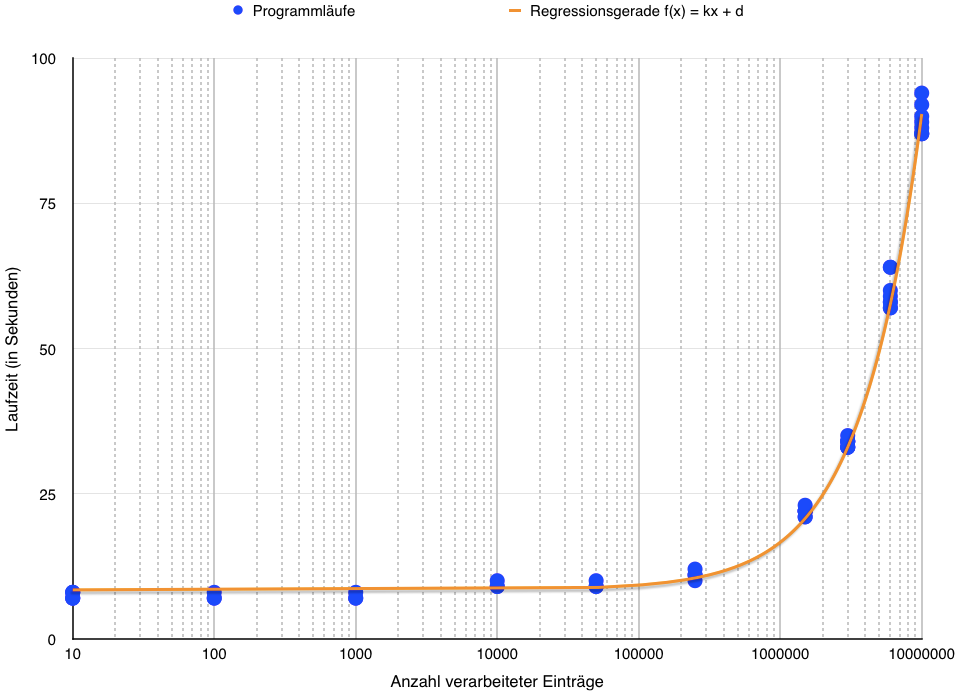
\includegraphics[width=1\textwidth]{Laufzeitanalyse.png}
	\caption{Verlauf der Regressionsgeraden}
	\label{fig:VerlaufRegressionsgerade}
\end{figure}

Um die ermittelte Funktion zu testen, wird nun zunächst die Laufzeit für die Verarbeitung von $2 \times 10^7$ Einträgen mit \autoref{equ:Laufzeit} berechnet. Anschließend wird die Anwendung mit der entsprechenden Anzahl von Einträgen zehn mal ausgeführt (siehe \autoref{lis:Laufzeit20Mio}), und die durchschnittliche Laufzeit mit der Berechnung verglichen. Die Dateigröße, bei $2 \times 10^7$ Einträgen, beträgt 3 \ac{GB}. \\

\begin{lstlisting}[language=Bash,caption=Laufzeiten mit $2 \times 10^7$ Einträgen,label=lis:Laufzeit20Mio]
Runtime: 185
Runtime: 171
Runtime: 166
Runtime: 174
Runtime: 166
Runtime: 172
Runtime: 170
Runtime: 170
Runtime: 171
Runtime: 171
\end{lstlisting}

Die Berechnete Laufzeit beträgt $t_e = 172,398$. Die durchschnittliche Laufzeit, bei 20 Mio. Einträgen, beträgt $171,6$. Die berechnete Laufzeit weicht lediglich $\approx 0,46\%$ vom Durchschnitt ab, was die Richtigkeit der Funktion hinreichend bestätigt.

\subsection{Definition des minimalen Ausführungsintervalls}
<Diese Zurückführung auf die Definition der maximalen Laufzeit funktioniert zwar, ist aber noch nicht richtig rund. Eventuell die Gleichung doch umschreiben. $t_e$ ist in der ursprünglichen Formel gesucht, wird hier jetzt aber teilweise gesucht und steht in der Definition als errechneter wert mit drin...das passt irgendwie noch nicht...>

In \autoref{subsubsec:PL001} wurde, durch die \autoref{equ:MaxAusführungszeit}, ein maximale Laufzeit für einen festen Ausführungsintervall definiert. Durch die Kombination mit \autoref{equ:Laufzeit}, durch welche sich ein zu erwartender Wert für $t_e$ berechnen lässt, kann die Definition um einen Gültigkeitsbereich für $t_i$ erweitern:

\begin{flalign}
&& && t_e \leq \frac{t_i}{5} && \{t_e \in \mathbb{Q}^+\},\;\{t_i \in \mathbb{N}\;|\;5t_e \leq t_i \leq +\infty\} \label{equ:MinInterval}
\end{flalign}

Durch diese Anpassung lässt sich, bereits vor Implementierung einer Analyse, ein minimaler Ausführungsintervall, in Abhängigkeit zur Datenmenge, bestimmen. Dies kann auch für bereits bestehende Analysen durchgeführt werden, um festzustellen, ob diese durch die Anwendung ersetzt werden können.

%<IDEE: Es wurde eine formel angegeben, welche aussage über die maximale ausführungsdauer gibt...eventuell lassen sich diese beiden formeln verbinden (also eine Formel die aussage gibt über den maximal möglichen intervall für eine bestimmte datenmenge \autoref{equ:MinInterval})>

%\begin{figure}
%	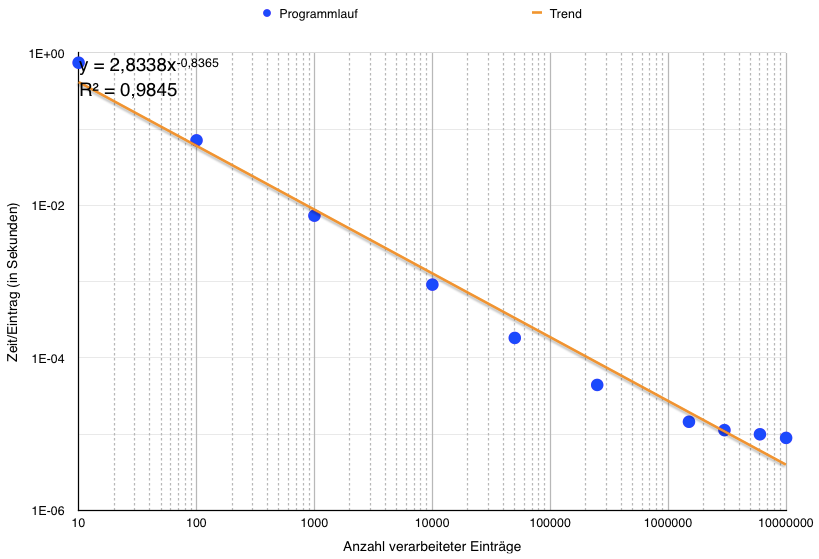
\includegraphics[width=1\textwidth]{Zeit_Pro_Eintrag.png}
%	\caption{Verarbeitungszeit pro Eintrag}
%	\label{fig:VerarbeitungszeitProEintrag}
%\end{figure}

%<Dokumentation der Tests mit unterschiedlich großen Datenmengen (10 Logeinträge bis 10.000.000 Einträge). Grafische Darstellung der Laufzeiten. Jede Stufe min. 10 mal ausführen und Ausführungszeit Nottieren/Dokumentieren. In Kapitel 6 Erkenntnisse aus den Tests aufarbeiten>